\section{Spherical Harmonics Analysis}
\label{sec:spherical_harmonics}

\subsection{Event Toplology and Spherical Harmonics}
\label{sec:topology_and_harmonics}
Signature of the 0{\nbb} decay is two electrons with total kinetic
energy equal to the isotope Q-value (e.g., 2.529~MeV for $^{130}$Te). These
two electrons are often above Cherenkov threshold and therefore will
produce two (fuzzy) rings of Cherenkov light on top of isotropic
scintillation light. $^{8}$B background events have only one electron
producing one Cherenkov ring.

In the detector regions where Cherenkov and scintillation light
overlap the Cherenkov light on average arrives earlier due to a time
delay in emission and a shorter wavelengths of the scintillation
light. Therefore, while a vast majority of light produced in
0{\nbb} decay events consists of scintillation photons, timing
information can be used to select a sample of photons with high
fraction of Cherenkov light.

Due to directional nature of the Cherenkov light the spatial
distribution of early photons on the detector sphere will be different
for the 0{\nbb} decay signal and the background from $^{8}$B events.



The simplest case for spherical harmonics analysis are events with the
vertex located exactly in the center of the detector. For such event
Cherenkov and scintillation light can be separated by applying a time
cut on the photon arrival time as demonstrated
in~\cite{Aberle2014}. To introduce the technique of spherical
harmonics analysis we will follow the same strategy as
in~\cite{Aberle2014} and use central events with a slightly
different cut on the photon arrival time of 33.5~ns.

In order to illustrate the difference between different event
topologies we introduce three event topologies: two electrons produced
back-to-back at 180$^{\circ}$ angle, two electrons at 90$^{\circ}$
angle, and a single electron. The two former are representative
topologies of the 0{\nbb} decay signal events and the latter represents
$^{8}$B background events. Figure~\ref{fig:Display_top_5MeV} shows
Cherenkov photon distributions of 5~MeV electrons for each of the
three topology. 100 events are overlayed in order to make Cherenkov
rings visible.

\begin{figure*}[h]
  \centering
  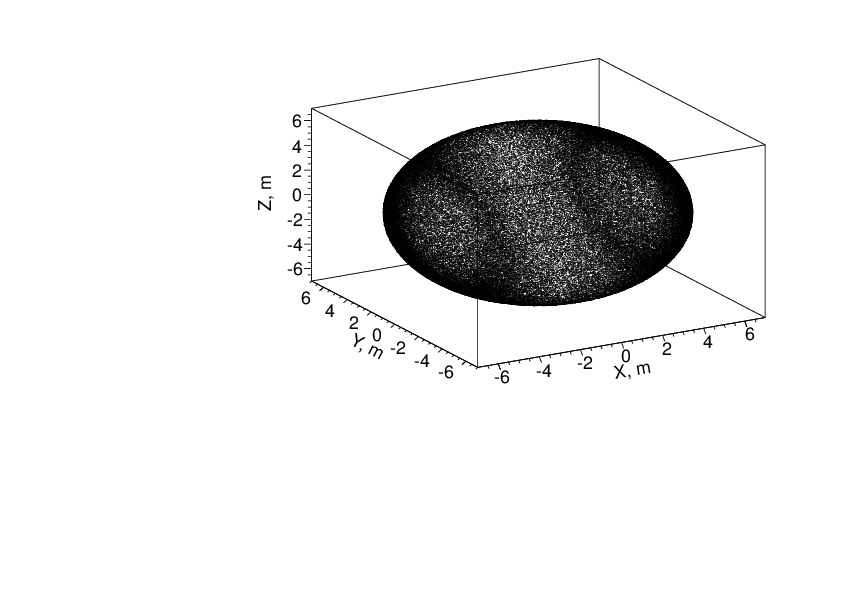
\includegraphics[width=0.3\textwidth]{hDisplay_topology180_5MeV.png}
  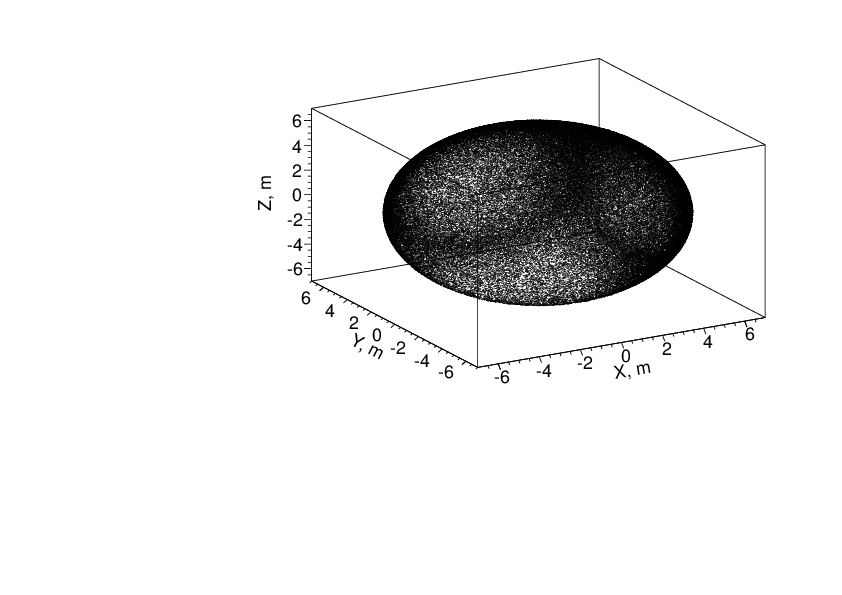
\includegraphics[width=0.3\textwidth]{hDisplay_topology90_5MeV.png}
  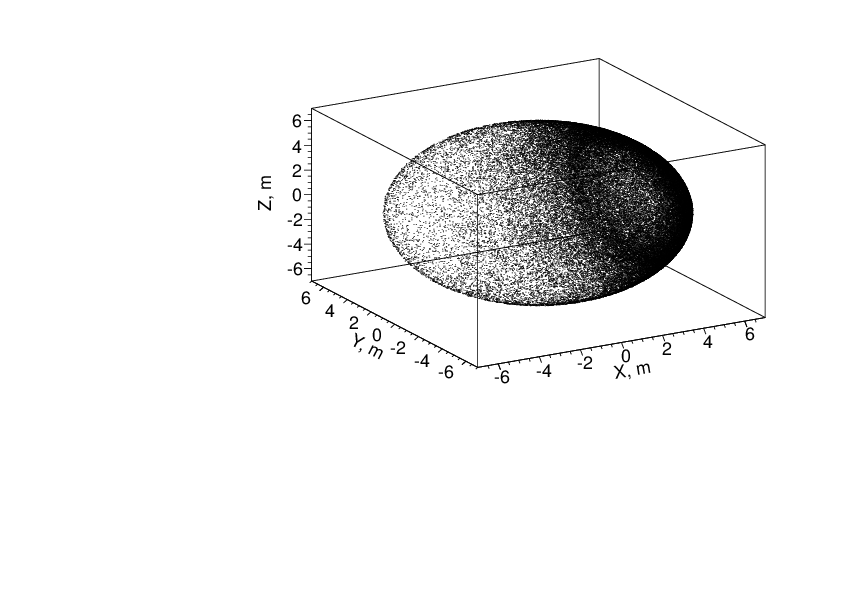
\includegraphics[width=0.3\textwidth]{hDisplay_1el_5MeV.png}
  \caption{Cherenkov photons distributions on the detector sphere for
    the three representative event topologies: two back-to-back
    electrons (\emph{left}), two electrons at 90$^{\circ}$ angle
    (\emph{middle}), and a single electron (\emph{center}).  All
    electrons are 5~MeV and originate at the center of the
    detector. 100 events overlayed for better visibility of the
    Cherenkov rings. 100\% QE is assumed. \JOcom{These can not be
      included as PDFs, but my conversion shrunk the size.}}
  \label{fig:Display_top_5MeV}
\end{figure*}

In practice Cherenkov rings from low energy electrons are not clearly
visible. Figure~\ref{fig:Display_top_2p5MeV} shows photons
distribution for individual events from three topologies with total
kinetic energy of 2.529~MeV (Q-value of $^{130}$Te). Event topology
can be identified by looking at clusters of Cherenkov photons in
different segments of the sphere.


\begin{figure*}[h]
  \centering
  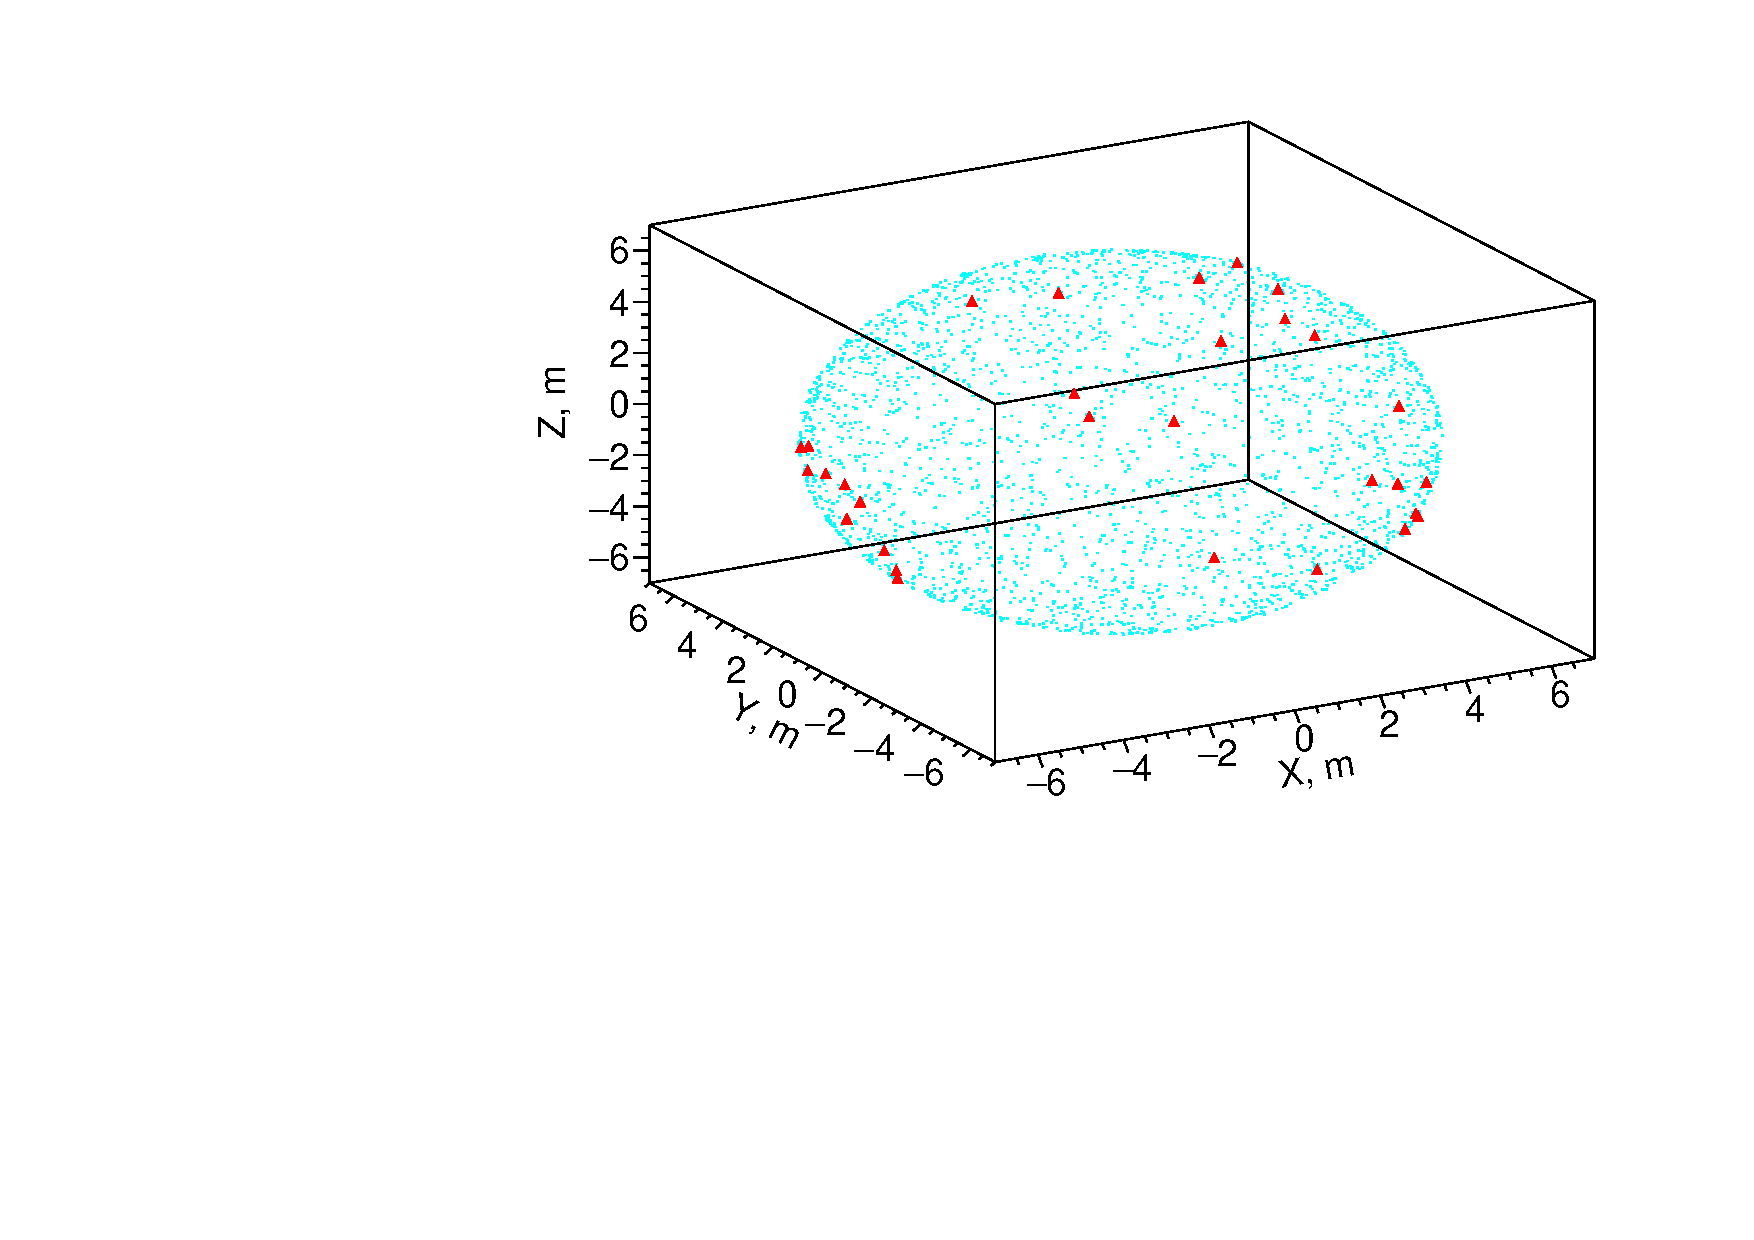
\includegraphics[width=0.3\textwidth]{hDisplay_topology180_2p529MeVTot}
  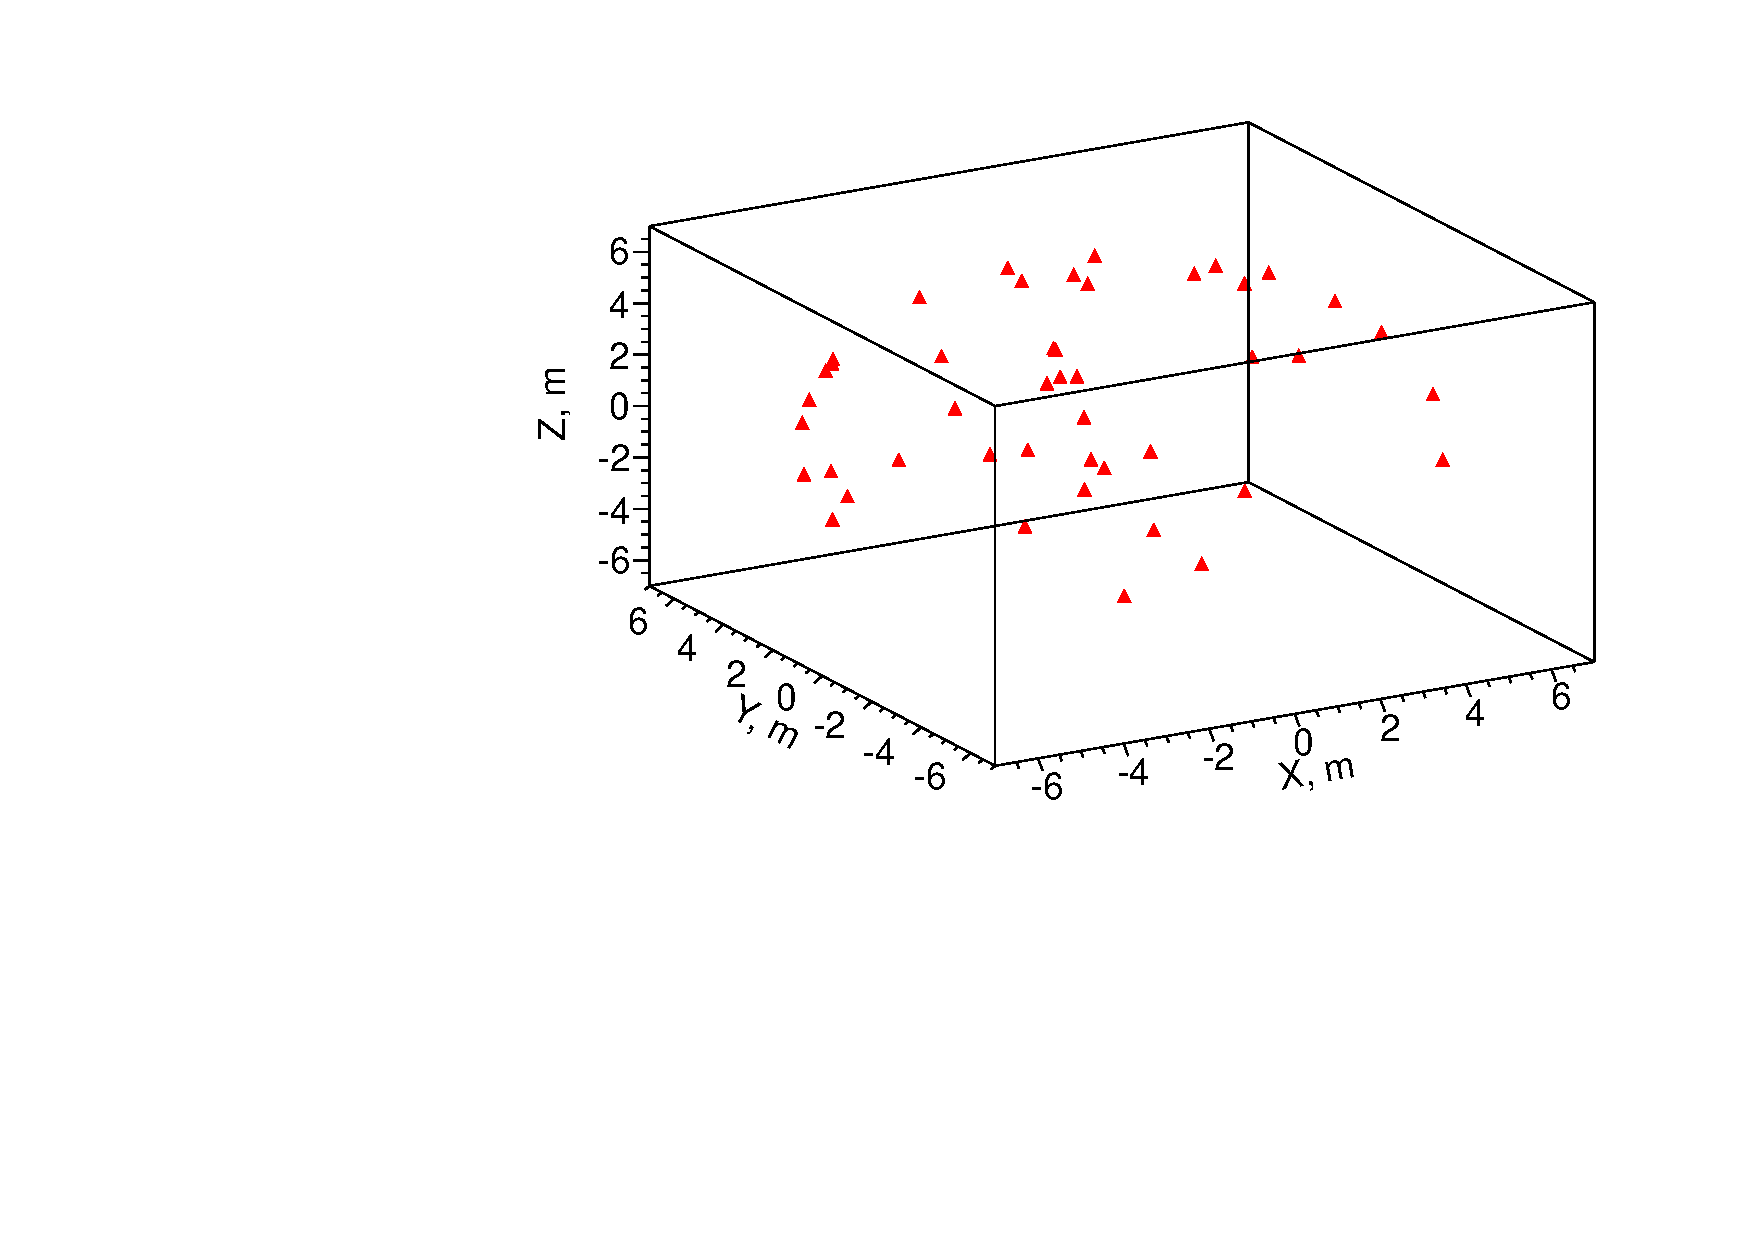
\includegraphics[width=0.3\textwidth]{hDisplay_topology90_2p529MeVTot}
  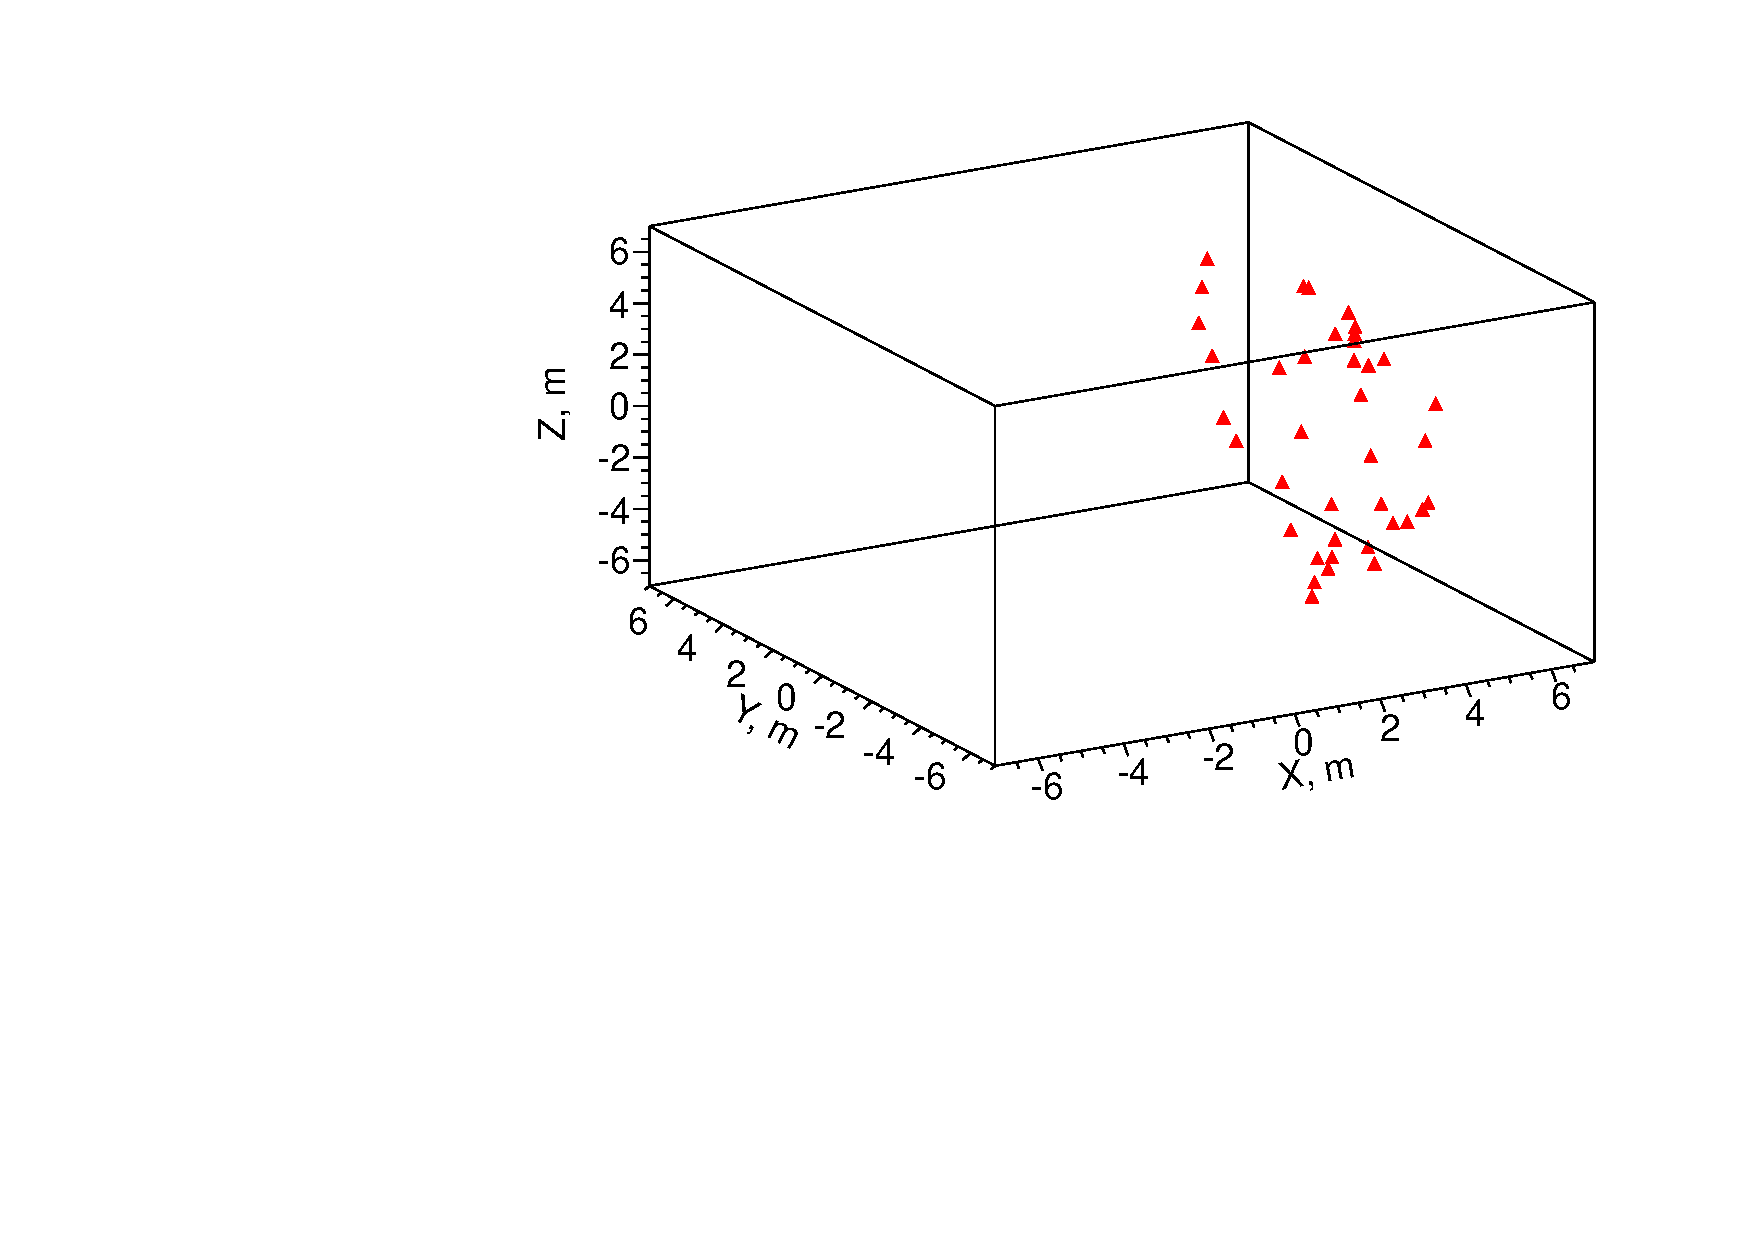
\includegraphics[width=0.3\textwidth]{hDisplay_1el_2p529MeV}
  \caption{Cherenkov photons distributions on the detector sphere for
    the three representative event topologies: two back-to-back 1.26~MeV
    electrons (\emph{left}), two 1.26~MeV electrons at 90$^{\circ}$
    angle (\emph{middle}), and a single 2.529~MeV electron
    (\emph{center}).  All electrons originate at the center of the
    detector. One randomly selected event is chosen for each
    category. Default QE is applied.}
  \label{fig:Display_top_2p5MeV}
\end{figure*}

Examples of three $^{130}$Te 0{\nbb} decay events simulated at the
center of the detector are shown in
Fig.~\ref{fig:Display_Te130}. Early PEs from Cherenkov and
scintillation light are shown. Default QE is used in the
simulation. Time cut of 33.5~ns on the photon arrival time is used to
select early light. Uniformly distributed scintillation light make it
more difficult to guess the event topology.  Nevertheless we show that
there is still sufficient difference in the position distribution of
the early light to separate two track and single track events.

\begin{figure*}[h]
  \centering
  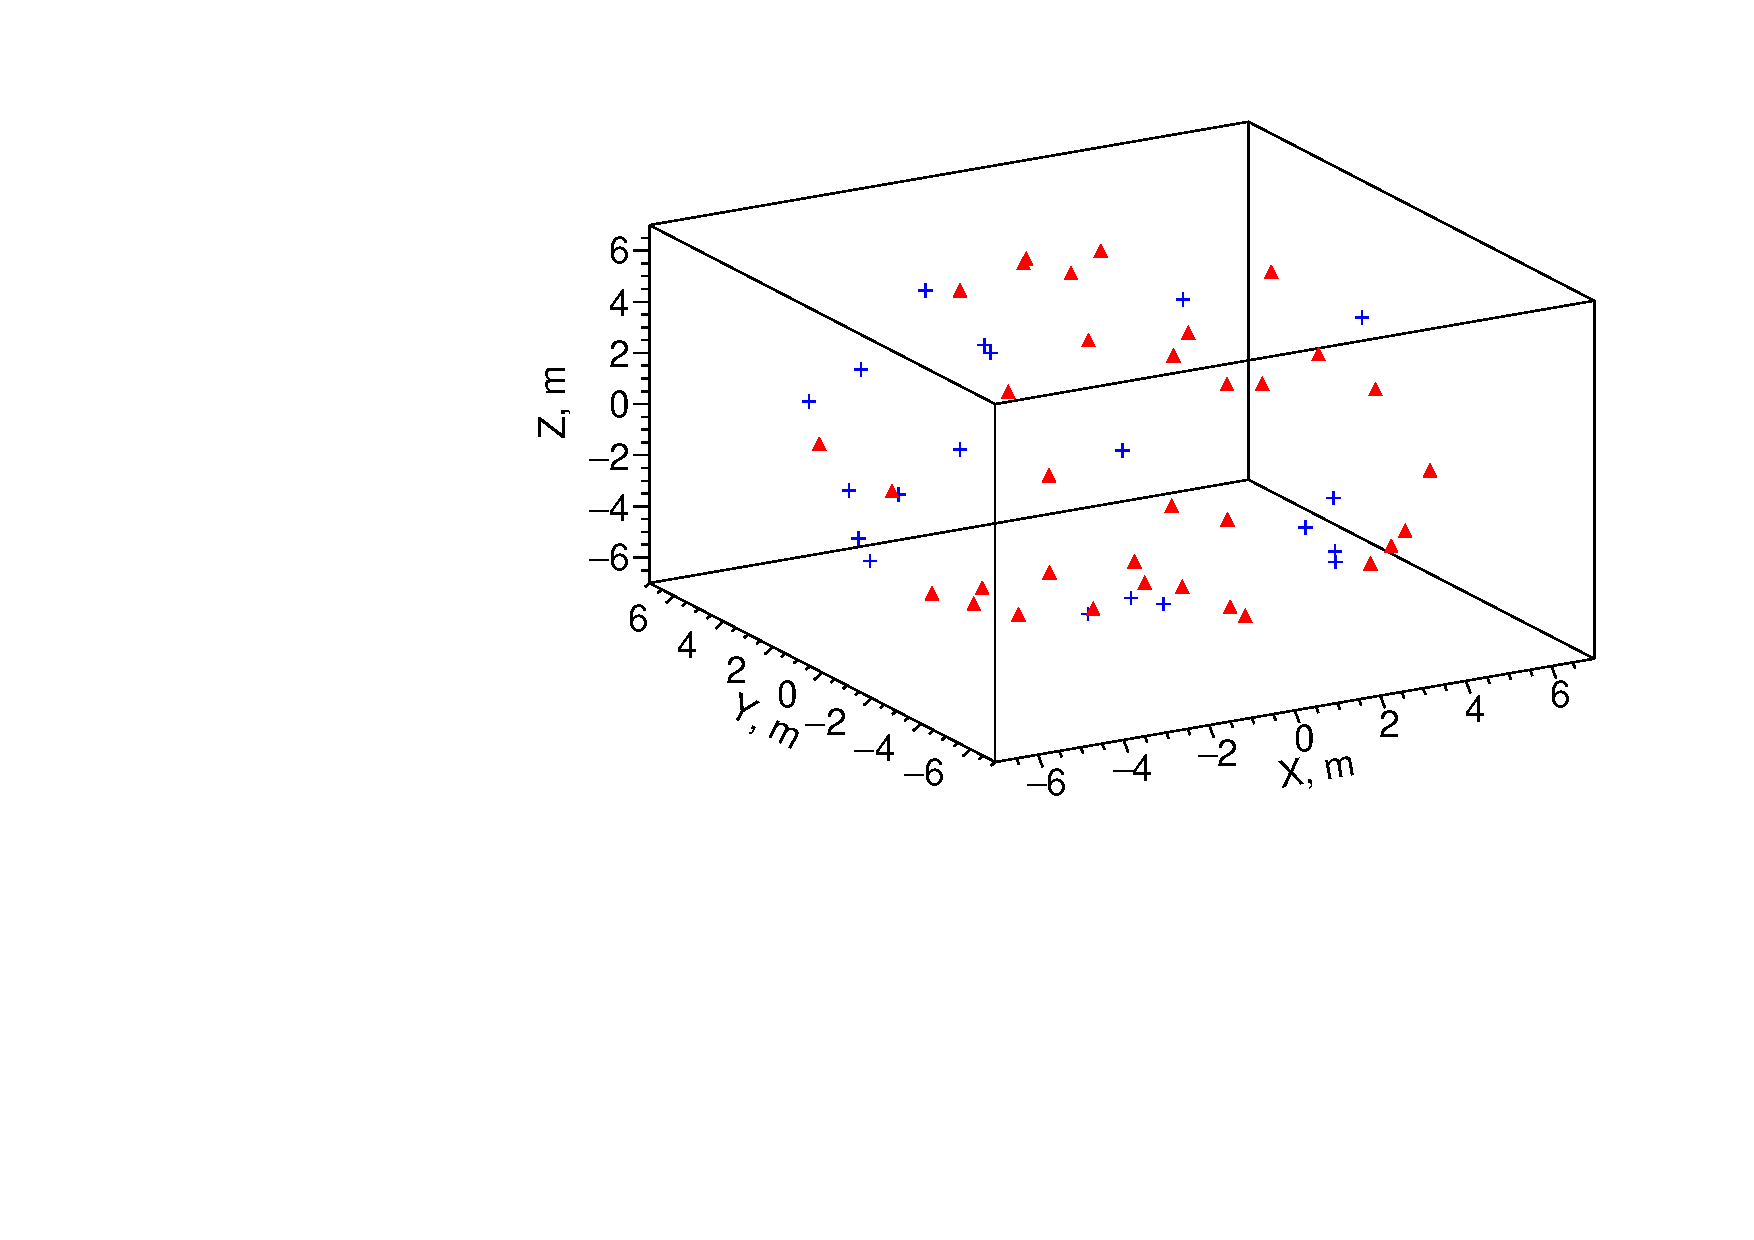
\includegraphics[width=0.45\textwidth]{hDisplay_Te130_evt124_e1257_e1270_cos-0908}
  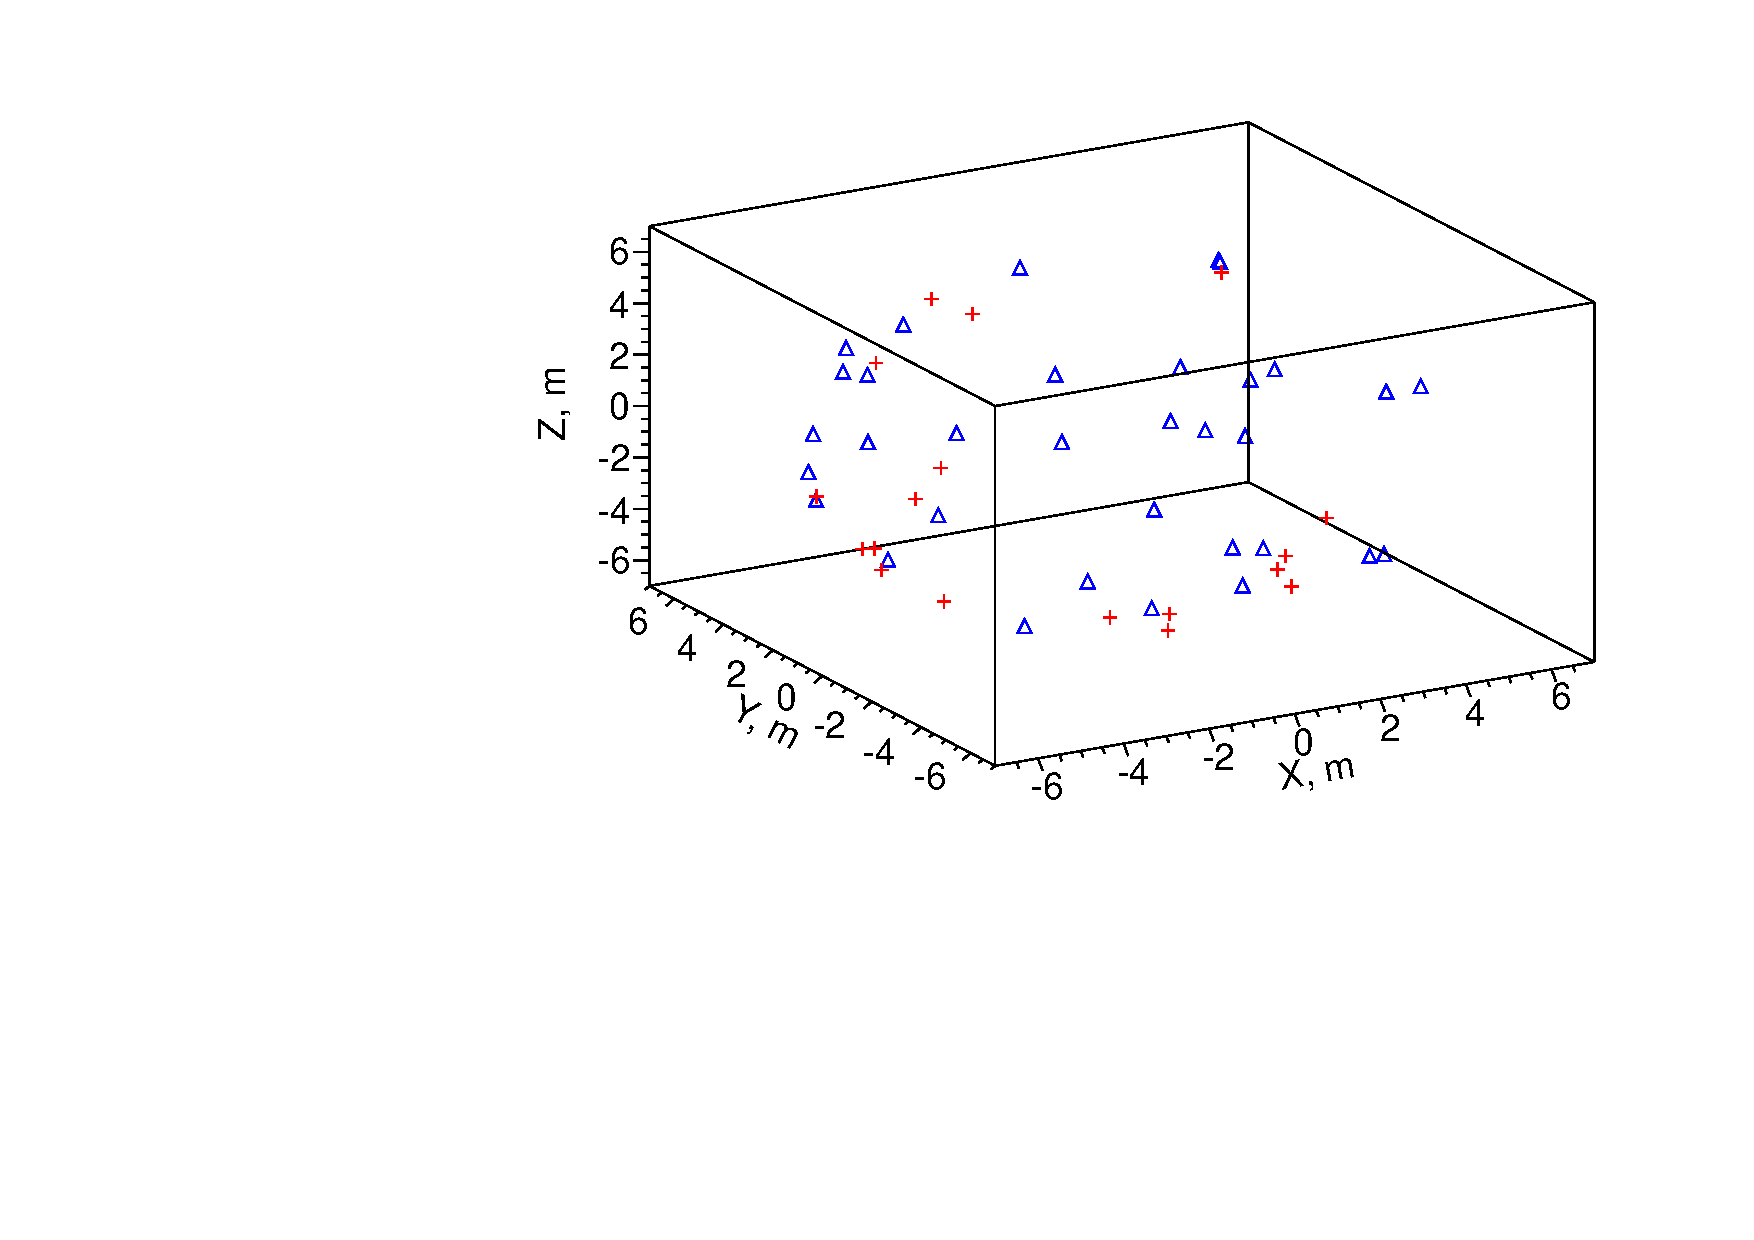
\includegraphics[width=0.45\textwidth]{hDisplay_Te130_evt131_e1264_e1263_cos-0029}
  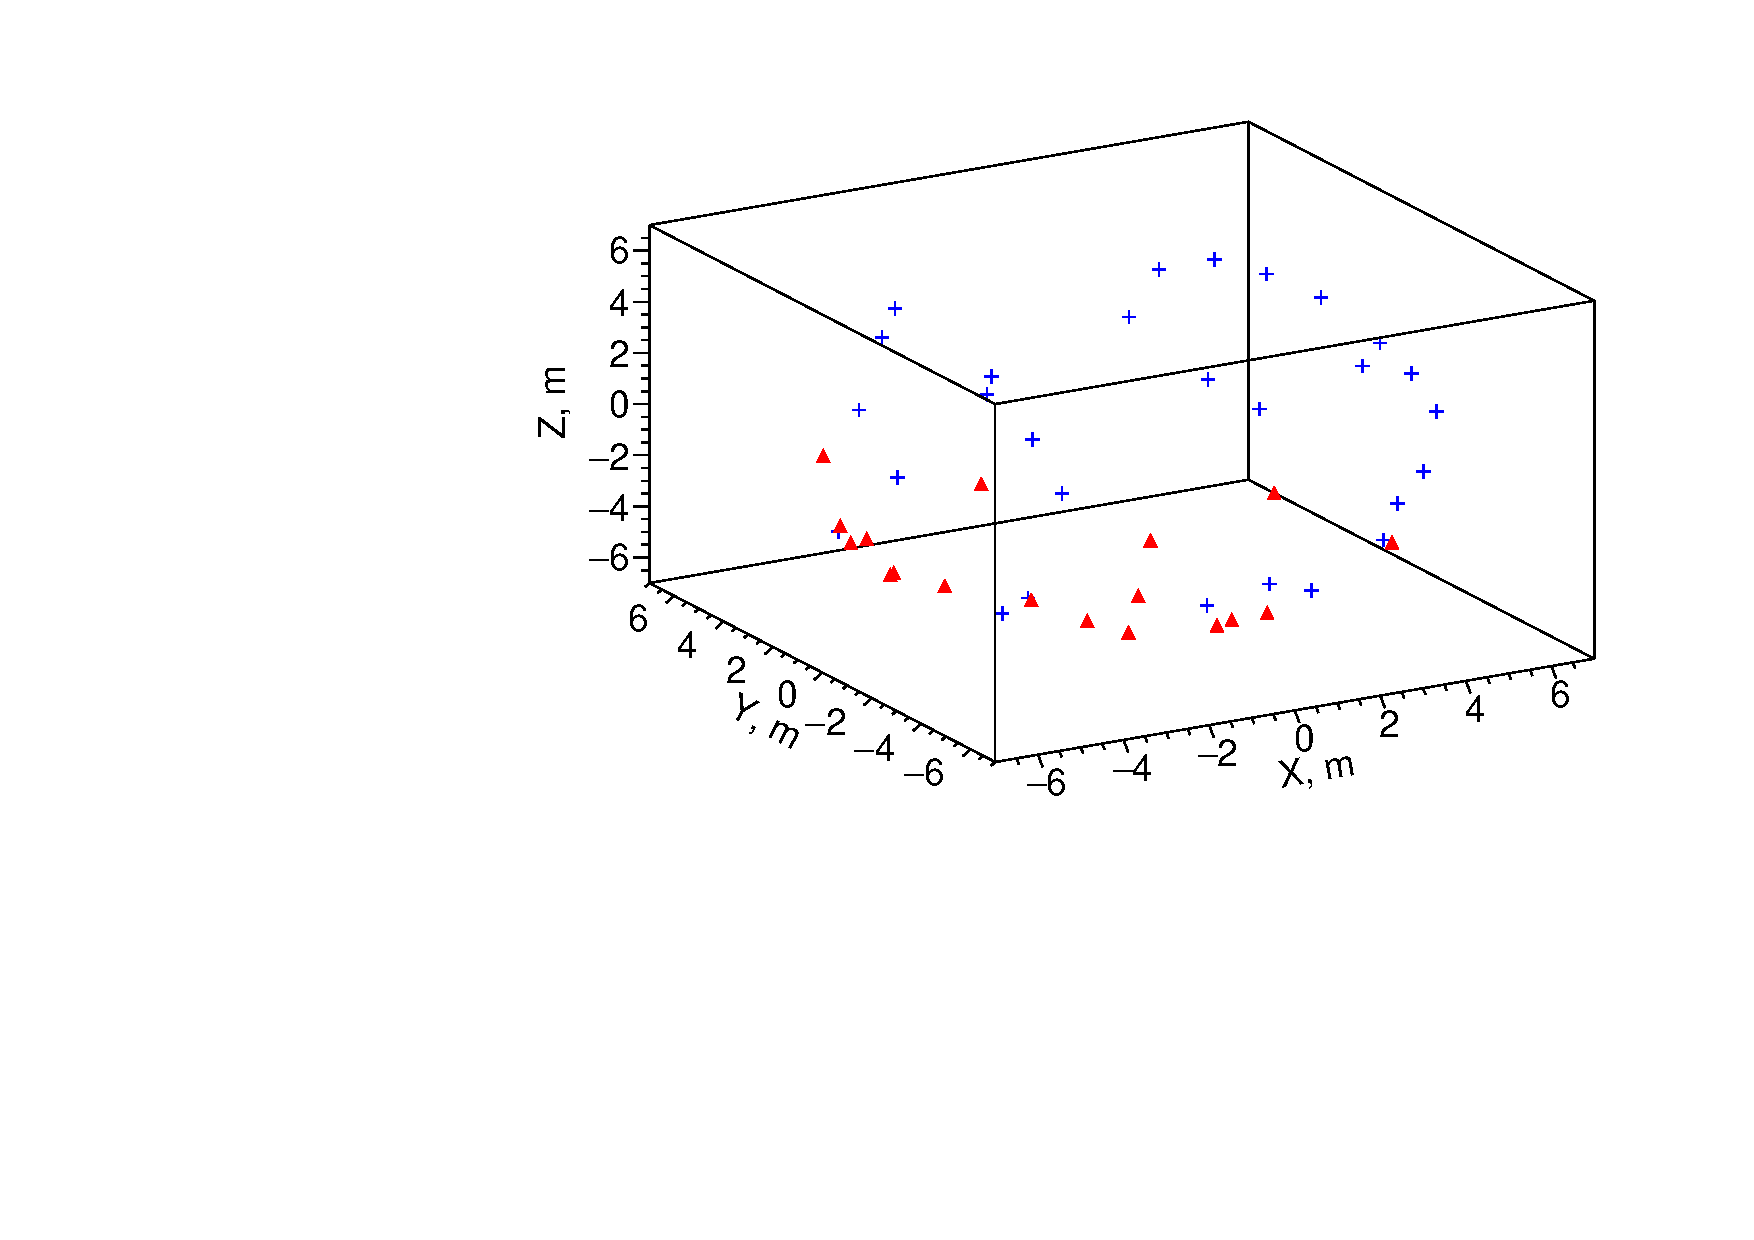
\includegraphics[width=0.45\textwidth]{hDisplay_Te130_evt352_e1186_e1340_cos0888}
  \caption{Examples of PEs position on the detector sphere after time
    cut of 33.5ns. PEs from Cherenkov (\emph{red}) and scintillation
    light (\emph{blue}) are compared. \emph{Top left:} $^{130}$Te
    0{\nbb} decay back-to-back electrons: $E_1$=1.257~MeV,
    $E_2$=1.270~MeV, cos($\theta$)=-0.908. \emph{Top right:}
    $^{130}$Te 0{\nbb} decay electrons at $\sim$90$^{\circ}$:
    $E_1$=1.264~MeV, $E_2$=1.263~MeV,
    cos($\theta$)=-0.029. \emph{Bottom left:} $^{130}$Te 0{\nbb} decay
    electrons at $\sim$0$^{\circ}$: $E_1$=1.186~MeV, $E_2$=1.340~MeV,
    cos($\theta$)=0.888. \emph{Bottom right:} 2.529~MeV single
    electron. Events are simulated at the center of the
    detector. Default QE is applied.}
\label{fig:Display_Te130}
\end{figure*}


0{\nbb} decay events become indistinguishable from single track
topology when the angle between two electrons is small For
quantitative description of the difference in the event topology we
analyze spherical harmonics of the photon distributions on the
detector sphere. We construct rotation invariant variables and compare
them between signal and background events. As it is shown in
Fig.~\ref{fig:Display_Te130} 0{\nbb} decay become indistinguishable
from single track topology when the angle between two electrons is
small (two degenerate tracks). Therefore the method of spherical
harmonics is most effective for events with large angular separation
between the two tracks.

In this paper we focus on topological difference between two tracks
and single track events and do not make any attempt to use absolute
directional information to suppress single track events which
direction is consistent with the direction from solar neutrinos. Once
a single track topology is established one can use a centroid method
(see Ref.~\cite{Aberle2014}) to reconstruct directionality of the
track or two degenerate tracks and get rid of events aligned with the
direction of $^{8}$B solar neutrinos.

\subsection{Mathematical description of spherical harmonics analysis}
A function $f(\theta,\phi)$ can be decomposed to a sum of spherical
harmonics:
\begin{eqnarray}
  \label{eq1}
  f(\theta,\phi) = \sum_{l=0}^{\infty} \sum_{m=-l}^{l} f_{lm}
  Y_{lm}(\theta,\phi),
\end{eqnarray}
where $Y_{lm}$ are Laplace's spherical harmonics defined in
Eq.~\ref{eq2} in real-value basis using Legendre polynomials
$P_l$. Coefficients $f_{lm}$ are defined in Eq.~\ref{eq3}
\begin{eqnarray}
  \label{eq2}
  Y_{lm} = LONGformulaHERE
\end{eqnarray}
\begin{eqnarray}
  \label{eq3}
  f_{lm} = LONGformulaHERE
\end{eqnarray}
Equation~\ref{eq4} defines multiple moments $S_l$ which are invariant
under rotation. Combination of $S_l$'s for ($l$=0,1,2...) is
determined by the event topology and can be used to distinguish
between different topologies.
\begin{eqnarray}
  \label{eq4}
  S_l = \sum_{m=-l}^{m=l} |f_{lm}|^2
\end{eqnarray}
Figure~\ref{fig:Moments} compares $S_l$ distributions for two
electrons emitted at 180 degree, two electrons at 90 degree, and a
single electron. Total kinetic energy of the electrons is the same in
all three cases.

\begin{figure*}[h]
  \centering
  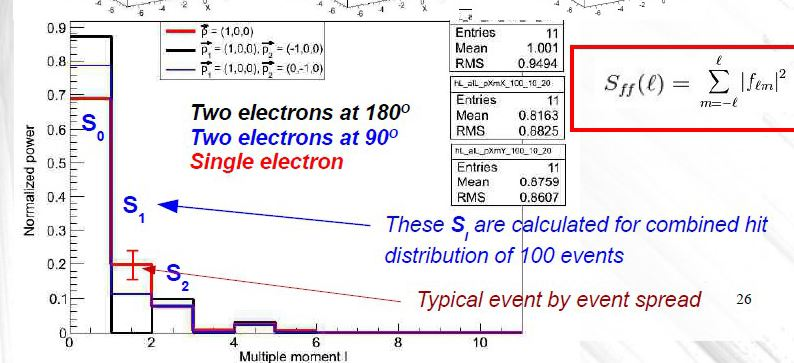
\includegraphics[width=0.95\textwidth]{Multiple_moment.JPG}
  \caption{Average $S_l$ values for two electrons at 180 degree
    (\emph{color1}) and 90 degree (\emph{color2}) 1.5~MeV each and a
    single electron (\emph{color3}) with the energy of 3~MeV. Error
    bars are RMS values of each corresponding individual $S_l$
    distribution (each consists of 1000 events simulated at the center
    of the detector) indicating typical event-by-event variation.}
\label{fig:Moments}
\end{figure*}


In order to compare spherical harmonics for events with vertices
located off-center anywhere inside the detector volume a coordinate
transformation for each photon hit is needed. The transformation
applied for each photon hit within an event is shown in
Fig.~\ref{fig:SphH_transform}. Solid circle schematically shows actual
detector boundaries. Dotted circle shows a new sphere of radius
R$=$6.5~m with the event vertex position in the center. The radius
vector of each photon hit is stretched or shorten until intersection
with this new sphere using transformation $\vec{r}^{,}_{hit} =
\frac{\vec{a}}{|\vec{a}|} \cdot R$. Where $\vec{r}^{,}_{hit}$ is a new
radius vector of the photon hit, R is detector sphere radius, and
$\vec{a}=\vec{r}_{hit} - \vec{r}_{vtx}$ with $\vec{r}_{hit}$ and
$\vec{r}_{vtx}$ being radius vectors of the photon hit and vertex
position in original coordinates.

\begin{figure*}[h]
  \centering
  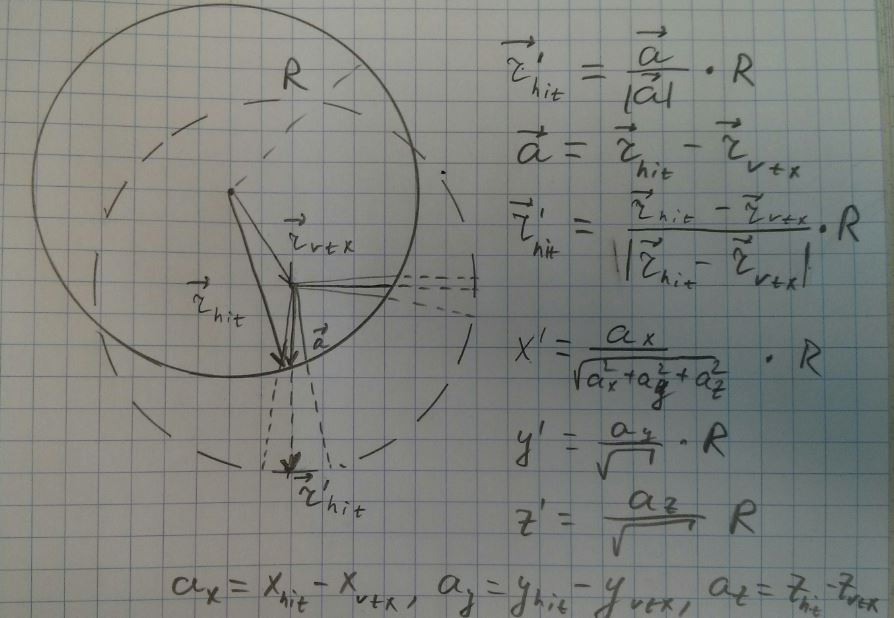
\includegraphics[width=0.95\textwidth]{plots/SphH_transform_sketch.JPG}
  \caption{Coordinate transformation applied to events that are
    off-center. Solid circle schematically shows actual detector
    boundaries. Dotted circle shows a new sphere of radius R$=$6.5~m
    with the event vertex position in the center. The radius vector of
    each photon hit is stretched or shorten until intersection with
    this new sphere using transformation $\vec{r}^{,}_{hit} =
    \frac{\vec{a}}{|\vec{a}|} \cdot R$. Where $\vec{r}^{,}_{hit}$ is a
    new radius vector of the photon hit, $R$ is detector sphere radius,
    and $\vec{a}=\vec{r}_{hit} - \vec{r}_{vtx}$ with $\vec{r}_{hit}$
    and $\vec{r}_{vtx}$ being radius vectors of the photon hit and
    vertex position in original coordinates and correspondingly.}
  \label{fig:SphH_transform}
\end{figure*}


\subsection{Software and implementation of the spherical harmonics analysis}
{\bf A few words on the implementation. Calculation of $S_l$'s
  requires numerical integration that needs to be explained.}

To illustrate spherical harmonics analysis technique we compare
distributions of $S_0$, $S_1$, $S_2$, and $S_3$ for the three
representative event topologies described in
Sec.~\ref{sec:topology_and_harmonics}. Almost all the information
about event topology is carried by Cherenkov light. Therefore we first
show spherical harmonics of back-to-back, 90$^{\circ}$ and single
track topologies calculated using Cherenkov light only (see
Fig.~\ref{fig:SL_topologies_CHE}). No is QE applied here.

Two top panels of Fig.~\ref{fig:SL_topologies_CHE} show 2-dimensional
distributions, S0 vs S1 and S2 vs S3, to demonstrate that all four
$S_l$'s provide separation between event topologies.  We also
introduce a 1-dimensional variable, S01 (bottom panel of
Fig.~\ref{fig:SL_topologies_CHE}), that has the best separation power
for majority of event topologies considered in this paper. $S_{01}$ is
defined as a projection of $S_1$ vs $S_2$ distribution onto a linear
fit of this 2-D distribution.

\begin{figure*}[h]
  \centering
  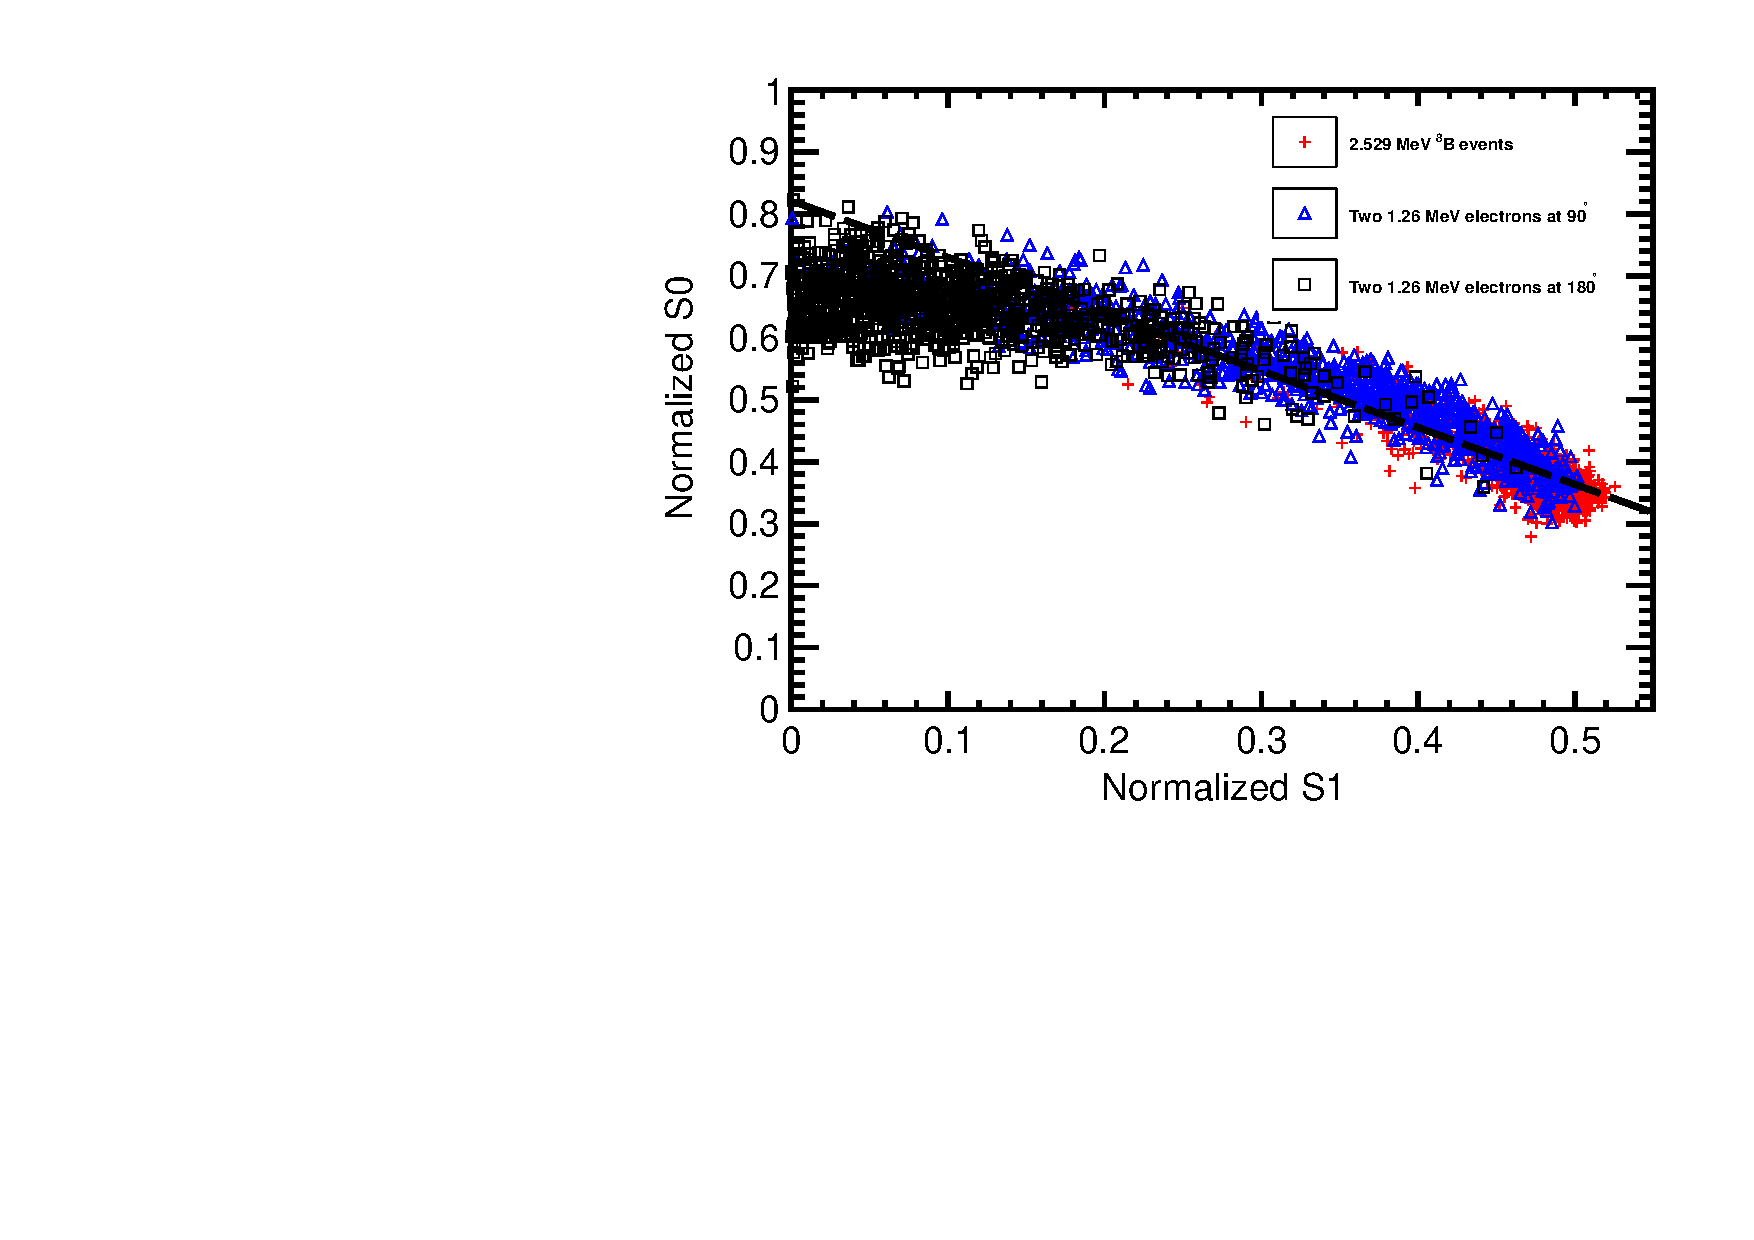
\includegraphics[width=0.49\textwidth]{plots/ALL/hS0vsS1_topologies_CHELight_VtxSmear0cm_VtxShiftX0cm_33p5ns_center.pdf}
  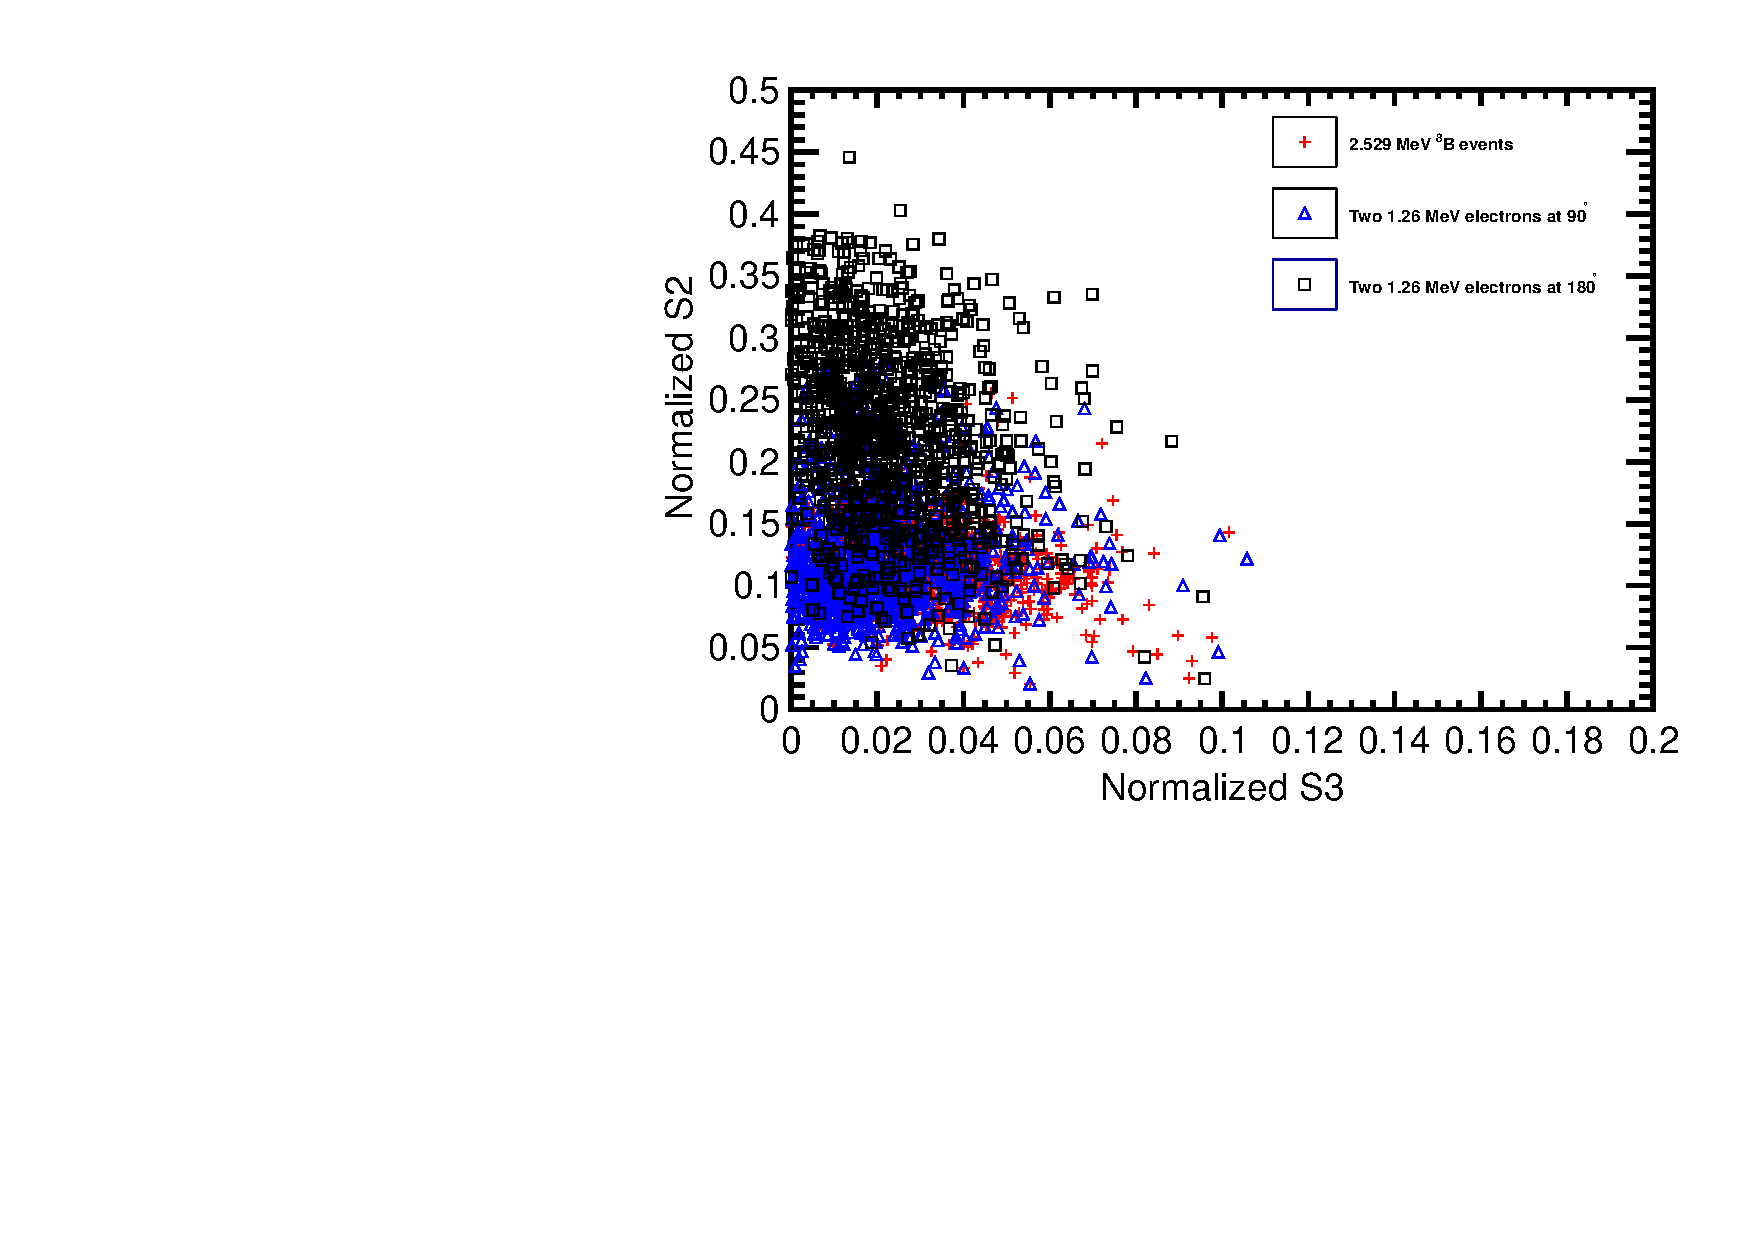
\includegraphics[width=0.49\textwidth]{plots/ALL/hS2vsS3_topologies_CHELight_VtxSmear0cm_VtxShiftX0cm_33p5ns_center.pdf}
  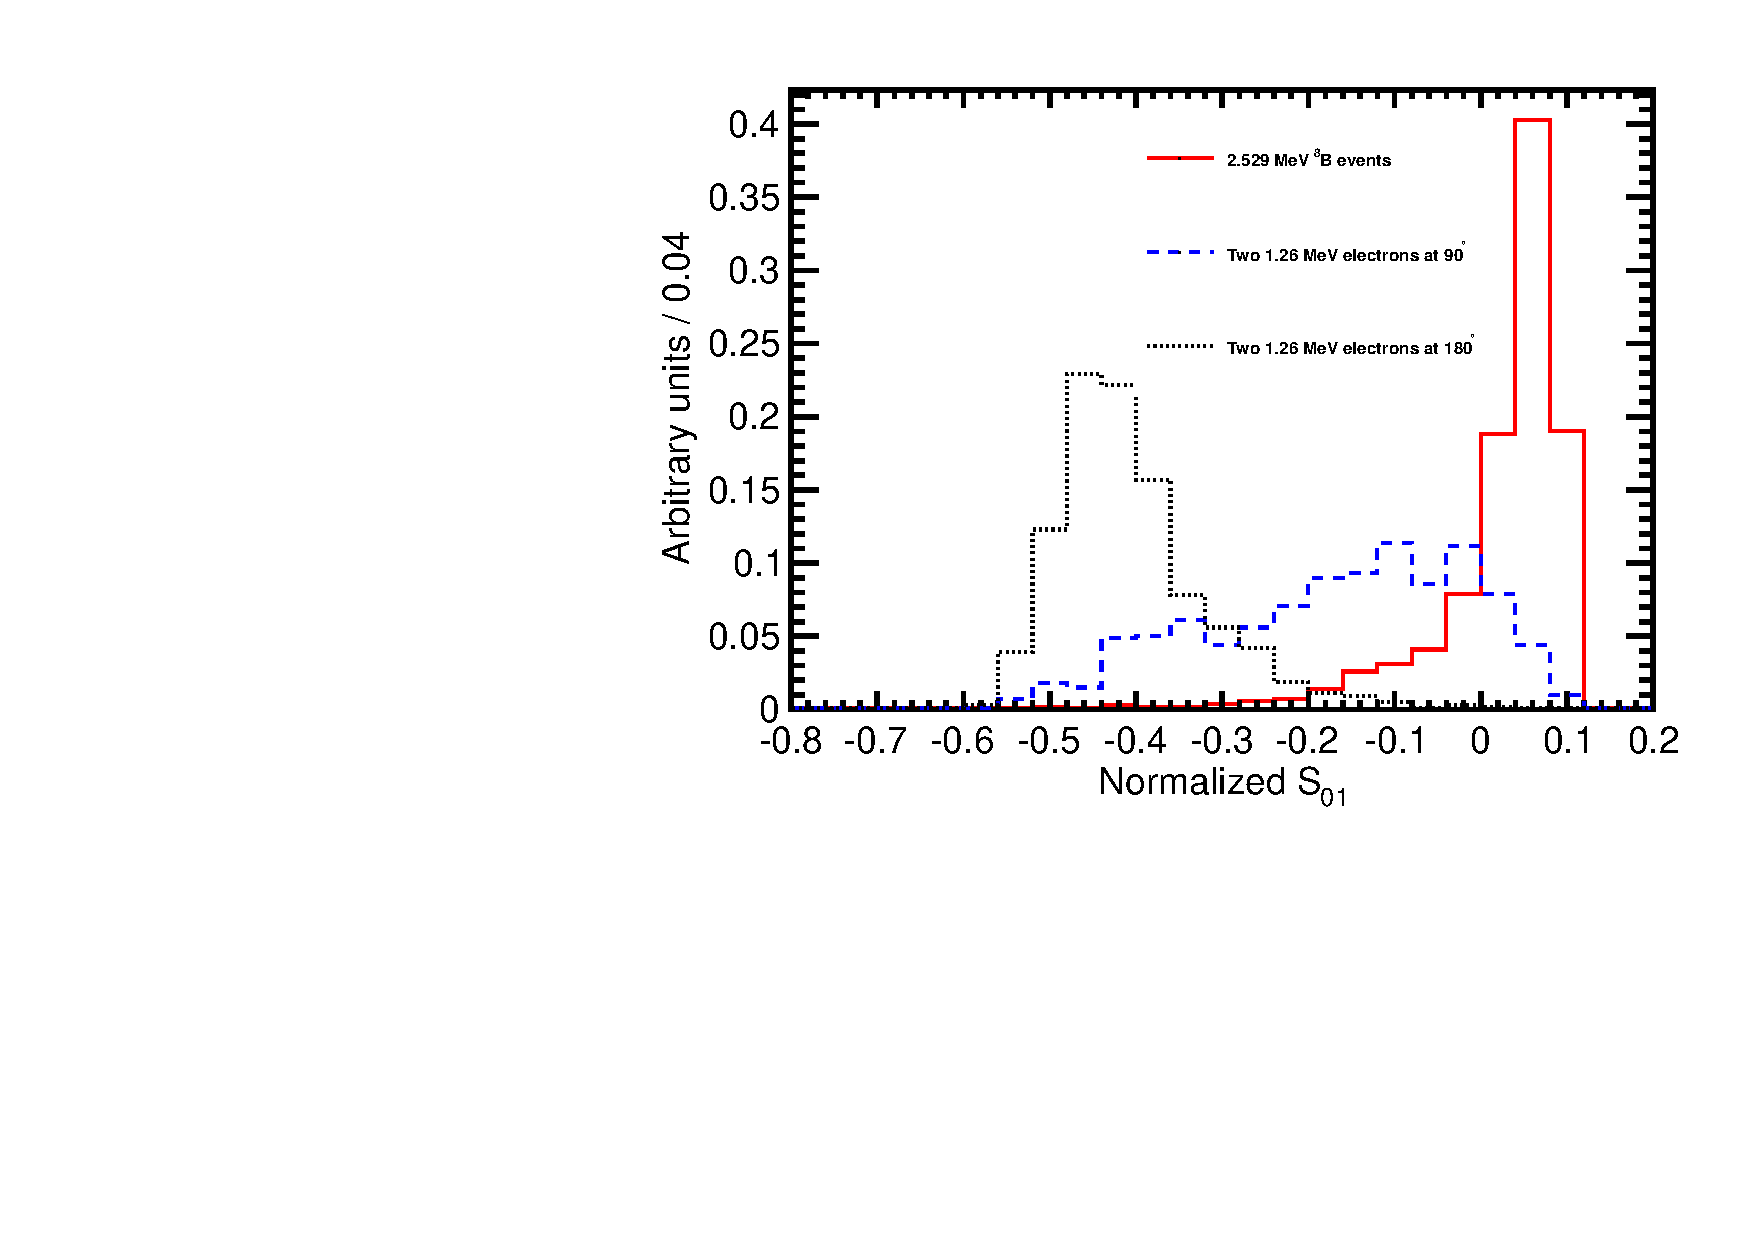
\includegraphics[width=0.9\textwidth]{plots/ALL/hS01_topologies_CHELight_VtxSmear0cm_VtxShiftX0cm_33p5ns_center.pdf}
  \caption{Spherical harmonics for three event topologies: two
    back-to-back 1.26~MeV electrons (\emph{black squares and black
      dotted line}), two 1.26~MeV electrons at 90$^{\circ}$ angle
    (\emph{blue triangles and blue dashed line}), and a single
    2.529~MeV electron representing $^{8}$B background (\emph{red
      crosses and red solid line}). Simulation of 1000 events
    originated at the center of the sphere. Perfect separation between
    Cherenkov and scintillation light is implemented in this
    simulation by using only Cherenkov photons. \emph{Top left:} $S_0$
    versus $S_1$ scatter plot. Black dotted line is a linear fit of
    the 90$^{\circ}$ topology and $^{8}$B events. Variable $S_{01}$ is
    defined as a projection of 2D distribution onto this linear
    fit. \emph{Top right:} $S_2$ versus $S_3$ scatter
    plot. \emph{Bottom:} $S_{01}$ distributions for the three
    topologies. These distributions are normalized to unit area for
    shape comparison.}
  \label{fig:SL_topologies_CHE}
\end{figure*}


The effects from scintillation light and applying default QE is shown
in Fig.~\ref{fig:SL_topologies_all}. Spherical harmonics of the same
three representative event topologies are now calculated using early
light (photons with arrival time less than 33.5~ns) that contains both
directional Cherenkov light and uniform scintillation light. Default
QE is also applied. Higher order multiple moments, S2 and S3, no
longer provide noticeable separation between different event
topologies.


\begin{figure*}[h]
  \centering
  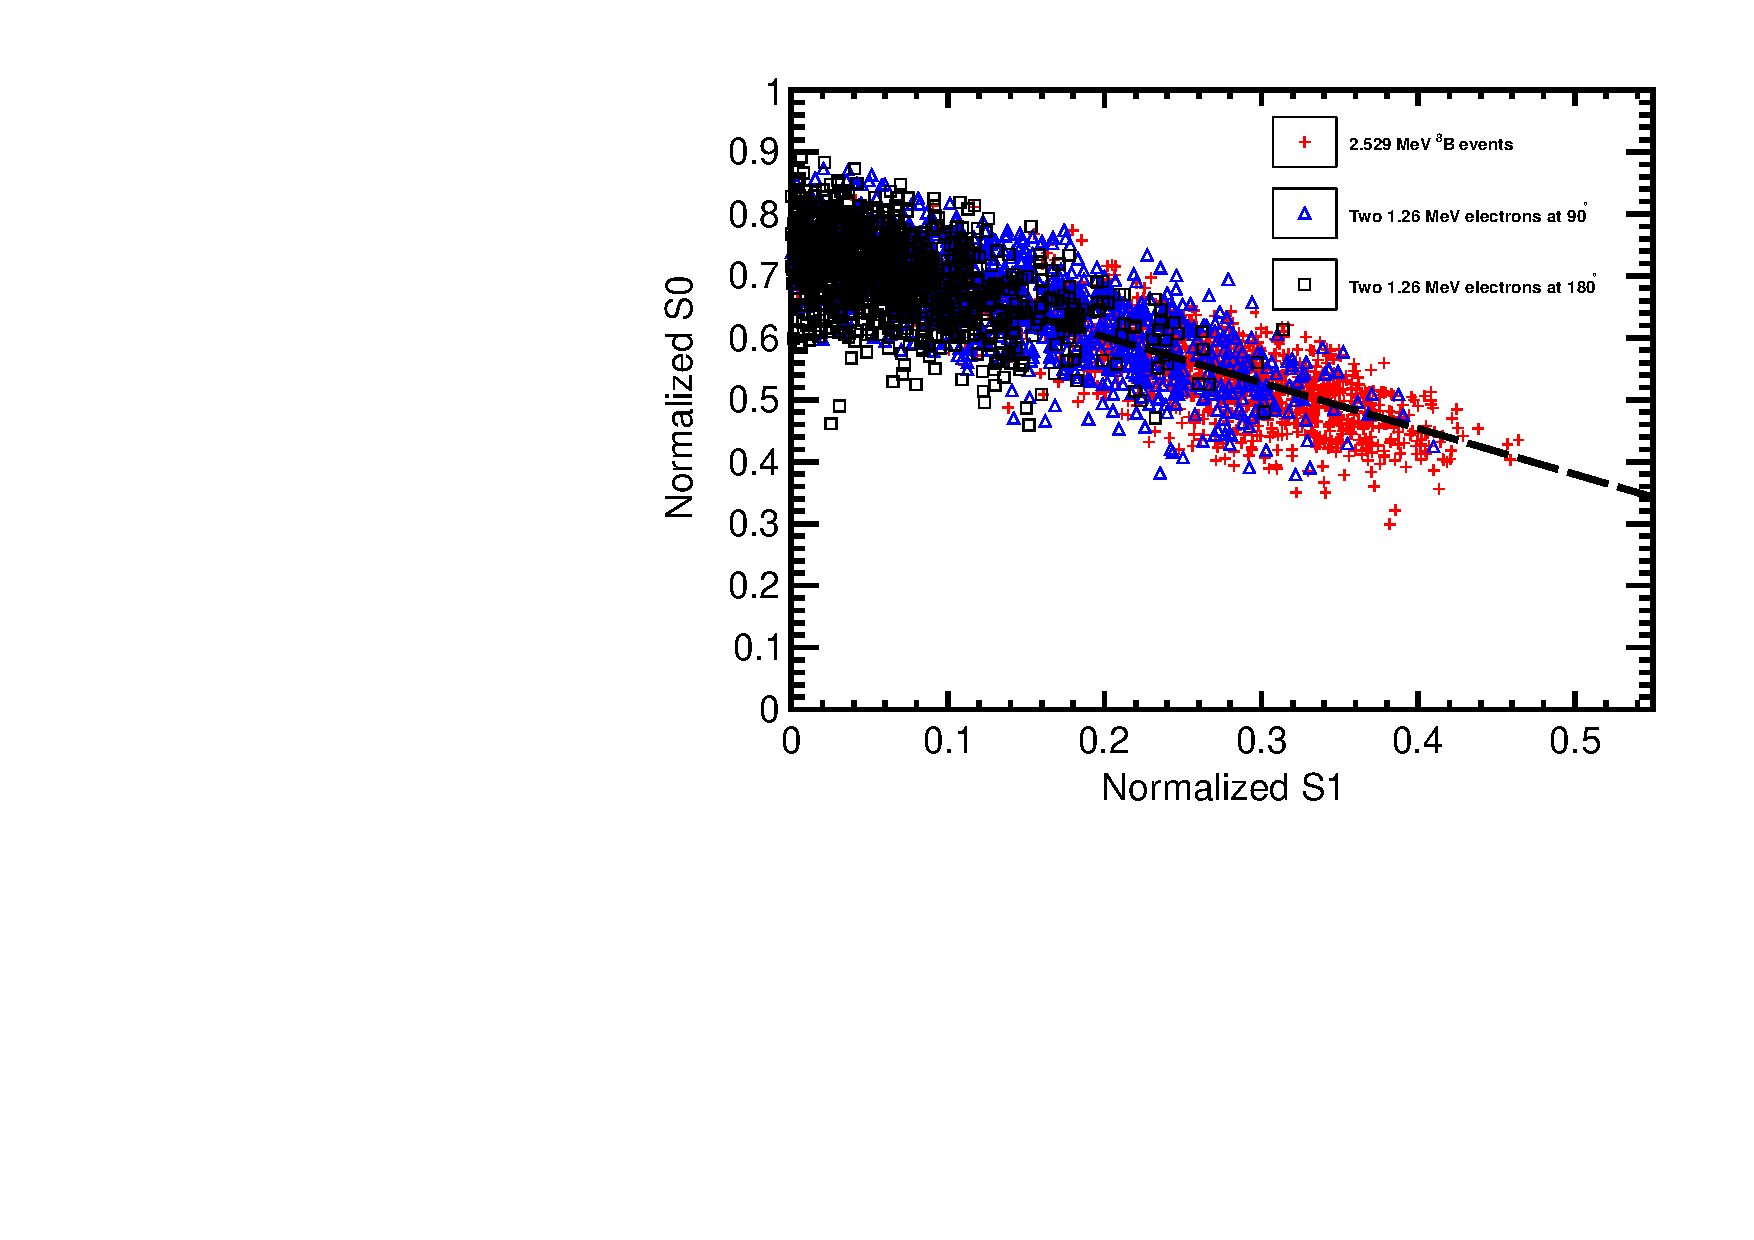
\includegraphics[width=0.49\textwidth]{plots/hS0vsS1_topologies_allLight_VtxSmear0cm_VtxShiftX0cm_33p5ns_center.pdf}
  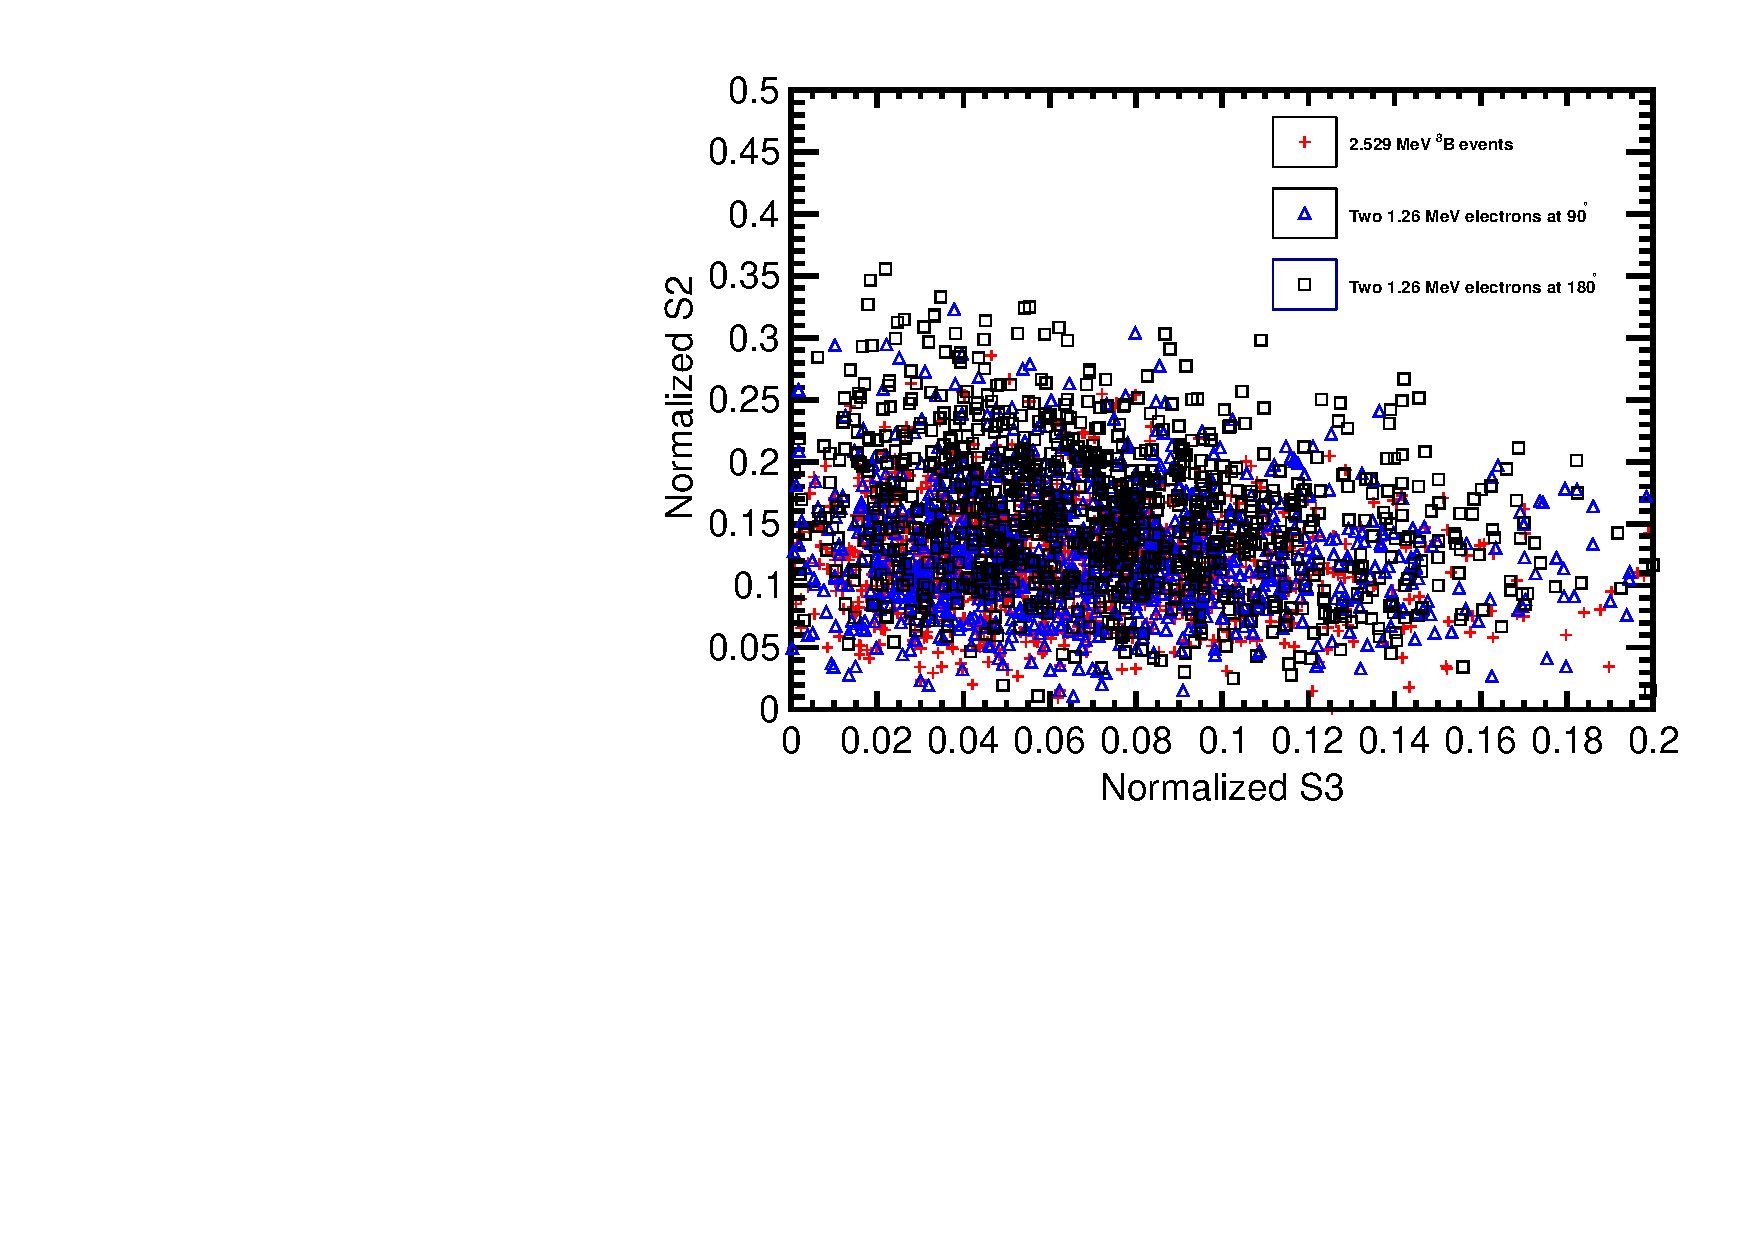
\includegraphics[width=0.49\textwidth]{plots/hS2vsS3_topologies_allLight_VtxSmear0cm_VtxShiftX0cm_33p5ns_center.pdf}
  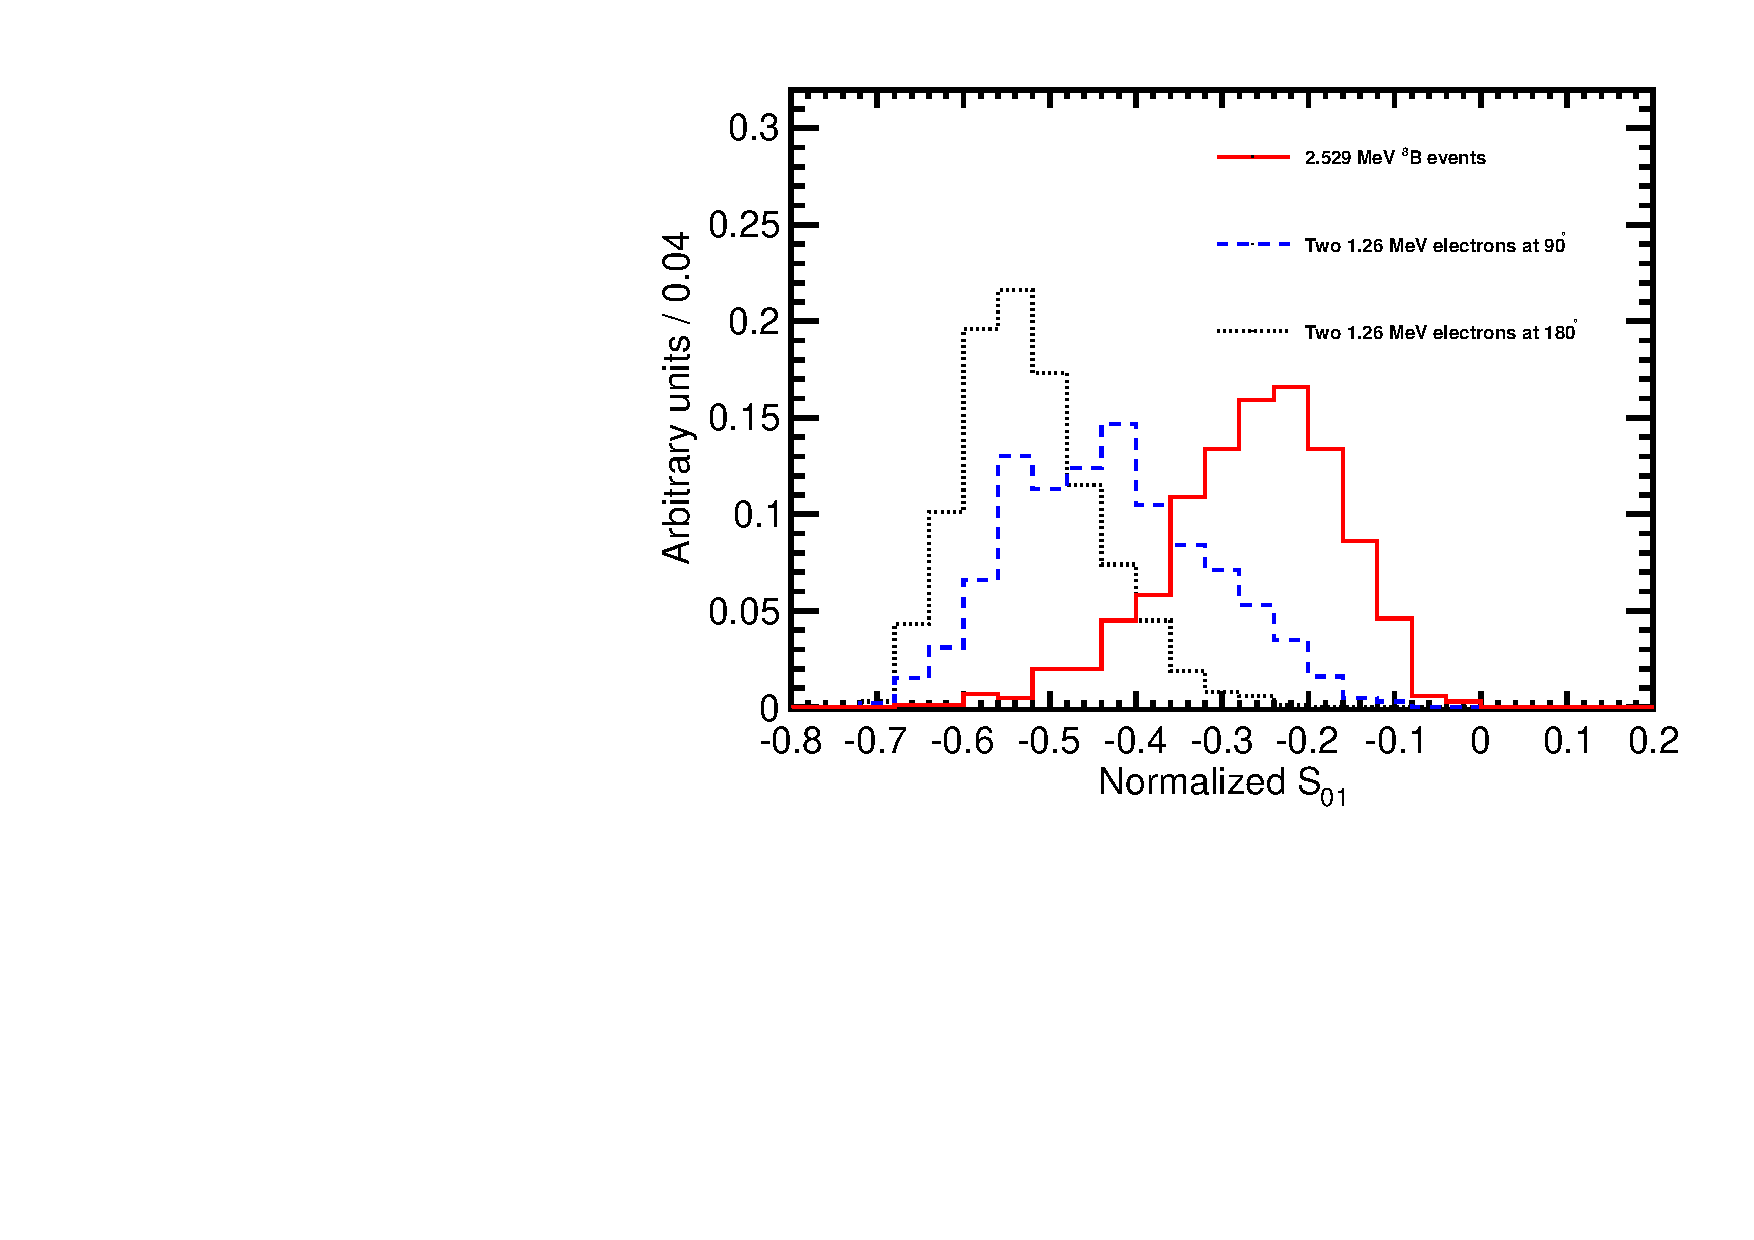
\includegraphics[width=0.9\textwidth]{plots/hS01_topologies_allLight_VtxSmear0cm_VtxShiftX0cm_33p5ns_center.pdf}
  \caption{Spherical harmonics for three event topologies: two
    back-to-back 1.26~MeV electrons (\emph{black squares and black
      dotted line}), two 1.26~MeV electrons at 90$^{\circ}$ angle
    (\emph{blue triangles and blue dashed line}), and a single
    2.529~MeV electron representing $^{8}$B background (\emph{red
      crosses and red solid line}). Simulation of 1000 events
    originated at the center of the sphere. Separation between
    Cherenkov and scintillation light is implemented 33.5~ns cut on
    the photon arrival time. Perfect vertex reconstruction - true
    vertex position is used. \emph{Top left:} $S_0$ versus $S_1$
    scatter plot. Black dotted line is a linear fit of the
    90$^{\circ}$ topology and $^{8}$B events. Variable $S_{01}$ is
    defined as a projection of 2D distribution onto this linear
    fit. \emph{Top right:} $S_2$ versus $S_3$ scatter
    plot. \emph{Bottom:} $S_{01}$ distributions for the three
    topologies. These distributions are normalized to unit area for
    shape comparison}
\label{fig:SL_topologies_all}
\end{figure*}

